\section{IrisEvent Class Reference}
\label{classIrisEvent}\index{IrisEvent@{IrisEvent}}
{\tt \#include $<$irisEvent.h$>$}

Collaboration diagram for IrisEvent:\nopagebreak
\begin{figure}[H]
\begin{center}
\leavevmode
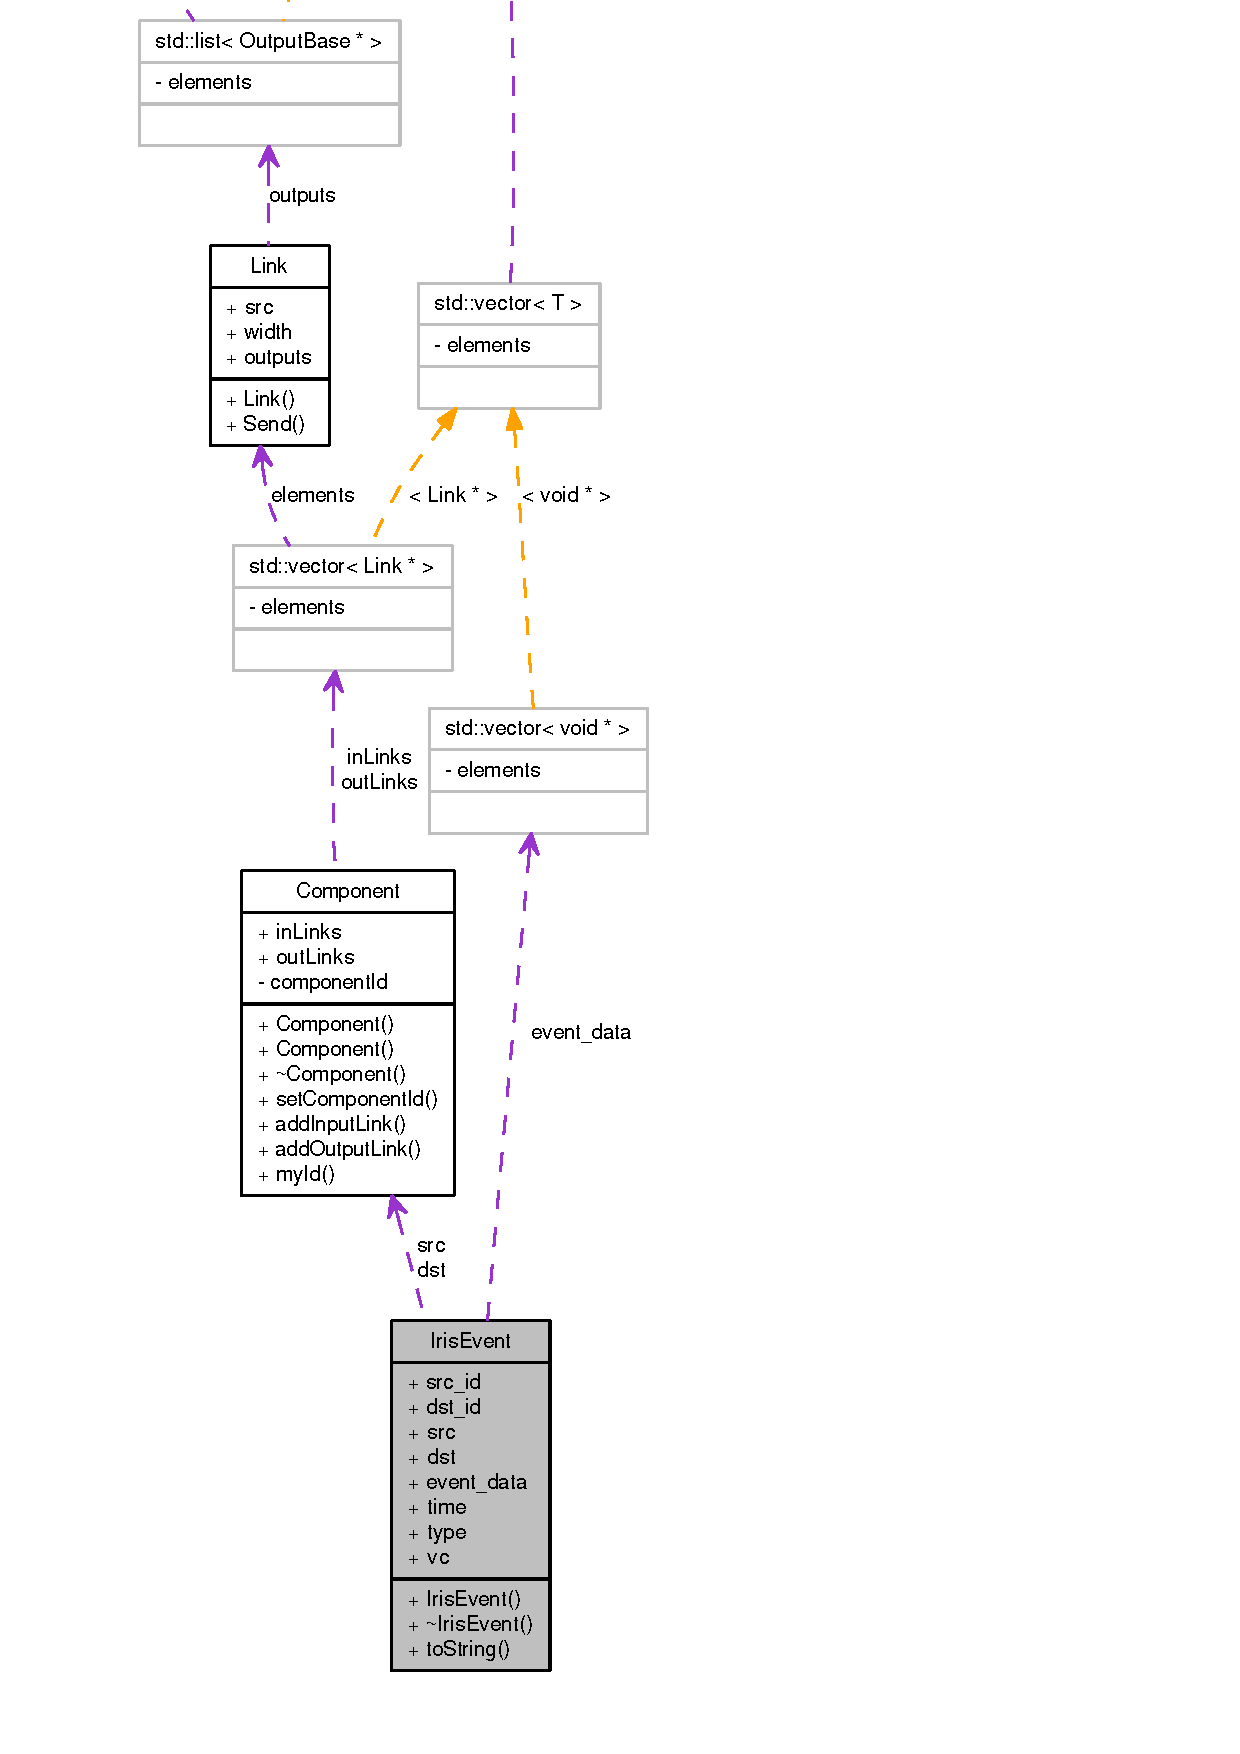
\includegraphics[height=400pt]{classIrisEvent__coll__graph}
\end{center}
\end{figure}
\subsection*{Public Member Functions}
\begin{CompactItemize}
\item 
{\bf IrisEvent} ()
\item 
{\bf $\sim$IrisEvent} ()
\item 
string {\bf toString} (void)
\end{CompactItemize}
\subsection*{Public Attributes}
\begin{CompactItemize}
\item 
{\bf uint} {\bf src\_\-id}
\item 
{\bf uint} {\bf dst\_\-id}
\item 
{\bf Component} $\ast$ {\bf src}
\item 
{\bf Component} $\ast$ {\bf dst}
\item 
vector$<$ void $\ast$ $>$ {\bf event\_\-data}
\item 
{\bf simTime} {\bf time}
\item 
{\bf uint} {\bf type}
\item 
{\bf uint} {\bf vc}
\end{CompactItemize}


\subsection{Detailed Description}


Definition at line 38 of file irisEvent.h.

\subsection{Constructor \& Destructor Documentation}
\index{IrisEvent@{IrisEvent}!IrisEvent@{IrisEvent}}
\index{IrisEvent@{IrisEvent}!IrisEvent@{IrisEvent}}
\subsubsection[{IrisEvent}]{\setlength{\rightskip}{0pt plus 5cm}IrisEvent::IrisEvent ()}\label{classIrisEvent_231a0a457b0f5469d17804d9ced7cc79}




Definition at line 35 of file irisEvent.cc.

References src\_\-id, and vc.\index{IrisEvent@{IrisEvent}!$\sim$IrisEvent@{$\sim$IrisEvent}}
\index{$\sim$IrisEvent@{$\sim$IrisEvent}!IrisEvent@{IrisEvent}}
\subsubsection[{$\sim$IrisEvent}]{\setlength{\rightskip}{0pt plus 5cm}IrisEvent::$\sim$IrisEvent ()}\label{classIrisEvent_5840e399aa6f659e30dc7757e71dc28b}




Definition at line 41 of file irisEvent.cc.

\subsection{Member Function Documentation}
\index{IrisEvent@{IrisEvent}!toString@{toString}}
\index{toString@{toString}!IrisEvent@{IrisEvent}}
\subsubsection[{toString}]{\setlength{\rightskip}{0pt plus 5cm}string IrisEvent::toString (void)}\label{classIrisEvent_0af2990076aab1512a61908435010824}




Definition at line 24 of file irisEvent.cc.

References Simulator::Now(), src\_\-id, and vc.

Referenced by NI::handle\_\-new\_\-packet\_\-event().

Here is the caller graph for this function:\nopagebreak
\begin{figure}[H]
\begin{center}
\leavevmode
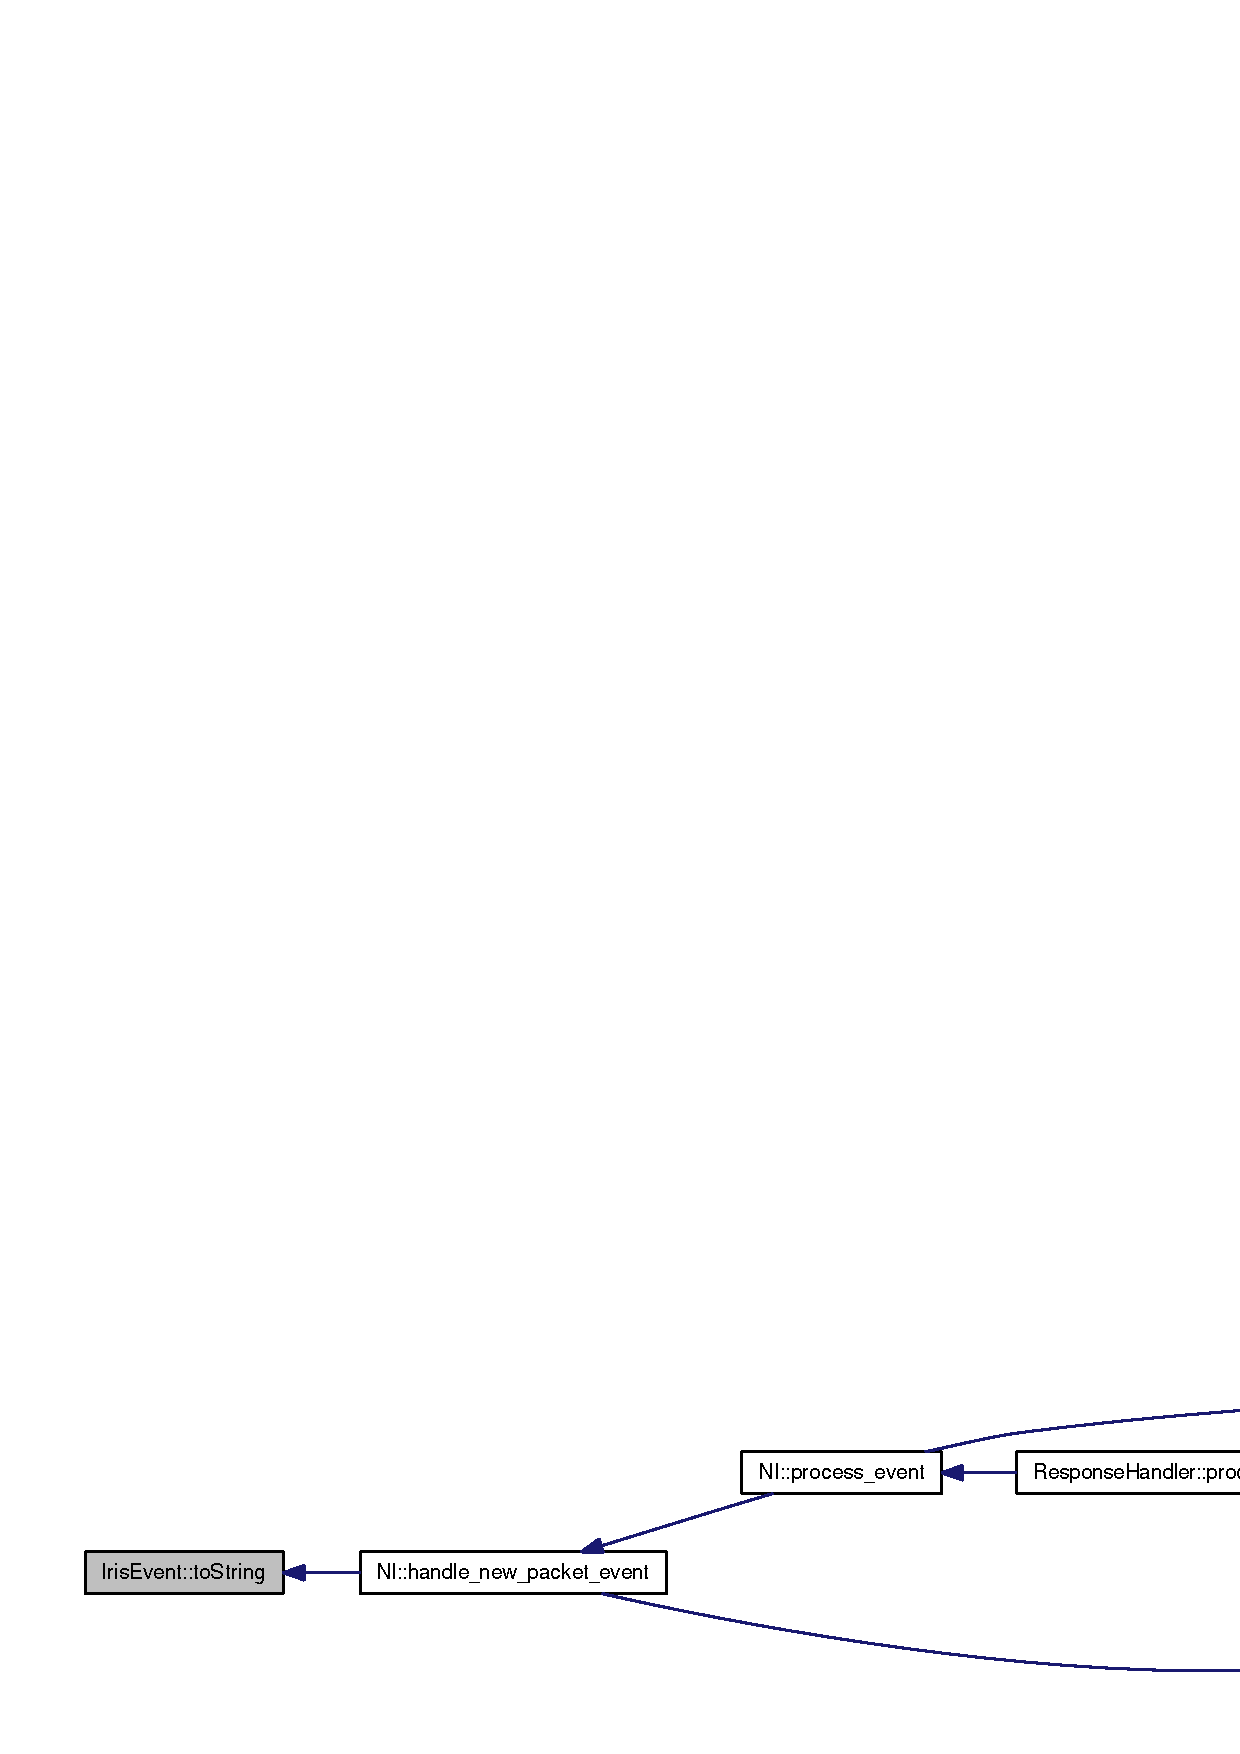
\includegraphics[width=420pt]{classIrisEvent_0af2990076aab1512a61908435010824_icgraph}
\end{center}
\end{figure}


\subsection{Member Data Documentation}
\index{IrisEvent@{IrisEvent}!dst@{dst}}
\index{dst@{dst}!IrisEvent@{IrisEvent}}
\subsubsection[{dst}]{\setlength{\rightskip}{0pt plus 5cm}{\bf Component}$\ast$ {\bf IrisEvent::dst}}\label{classIrisEvent_dbc9bf0bf1b6c36e3513cc4acde2e8dc}




Definition at line 46 of file irisEvent.h.

Referenced by NI::handle\_\-new\_\-packet\_\-event(), NI::handle\_\-out\_\-pull\_\-event(), main(), ResponseHandler::process\_\-event(), RefreshMgr::process\_\-event(), MSHR\_\-H::process\_\-event(), CmdIssuer::process\_\-event(), BankHandler::process\_\-event(), and MC::sim\_\-main().\index{IrisEvent@{IrisEvent}!dst\_\-id@{dst\_\-id}}
\index{dst\_\-id@{dst\_\-id}!IrisEvent@{IrisEvent}}
\subsubsection[{dst\_\-id}]{\setlength{\rightskip}{0pt plus 5cm}{\bf uint} {\bf IrisEvent::dst\_\-id}}\label{classIrisEvent_274c046ce64d15b914c0b8cbdebfea31}




Definition at line 44 of file irisEvent.h.

Referenced by GenericLink::handle\_\-link\_\-arrival\_\-event().\index{IrisEvent@{IrisEvent}!event\_\-data@{event\_\-data}}
\index{event\_\-data@{event\_\-data}!IrisEvent@{IrisEvent}}
\subsubsection[{event\_\-data}]{\setlength{\rightskip}{0pt plus 5cm}vector$<$void $\ast$$>$ {\bf IrisEvent::event\_\-data}}\label{classIrisEvent_26464fd0f931717a1e83b91111efc7b4}




Definition at line 47 of file irisEvent.h.

Referenced by GenericInterfaceVcs::handle\_\-link\_\-arrival(), GenericInterface::handle\_\-link\_\-arrival(), GenericRouterVct::handle\_\-link\_\-arrival\_\-event(), GenericRouterVcs::handle\_\-link\_\-arrival\_\-event(), GenericRouterNoVcs::handle\_\-link\_\-arrival\_\-event(), GenericLink::handle\_\-link\_\-arrival\_\-event(), GenericRouterAdaptive::handle\_\-link\_\-arrival\_\-event\_\-multiple\_\-flit\_\-in\_\-buffer(), GenericRouterAdaptive::handle\_\-link\_\-arrival\_\-event\_\-one\_\-msg\_\-per\_\-buffer(), uncore\_\-t::handle\_\-new\_\-packet\_\-event(), NI::handle\_\-new\_\-packet\_\-event(), GenericTPGVcs::handle\_\-new\_\-packet\_\-event(), GenericTPG::handle\_\-new\_\-packet\_\-event(), GenericSink::handle\_\-new\_\-packet\_\-event(), GenericRPG::handle\_\-new\_\-packet\_\-event(), GenericInterfaceVcs::handle\_\-new\_\-packet\_\-event(), GenericInterface::handle\_\-new\_\-packet\_\-event(), GenericFlatMc::handle\_\-new\_\-packet\_\-event(), GenericSink::handle\_\-ready\_\-event(), GenericRPG::handle\_\-ready\_\-event(), GenericInterfaceVcs::handle\_\-tick\_\-event(), GenericInterface::handle\_\-tick\_\-event(), main(), ResponseHandler::process\_\-event(), RequestHandler::process\_\-event(), MSHR\_\-SA\_\-H::process\_\-event(), MSHR\_\-H::process\_\-event(), DRAMChannel::process\_\-event(), DataBusHandler::process\_\-event(), CmdIssuer::process\_\-event(), CmdBusHandler::process\_\-event(), BankHandler::process\_\-event(), GenericSink::setup(), and MC::sim\_\-main().\index{IrisEvent@{IrisEvent}!src@{src}}
\index{src@{src}!IrisEvent@{IrisEvent}}
\subsubsection[{src}]{\setlength{\rightskip}{0pt plus 5cm}{\bf Component}$\ast$ {\bf IrisEvent::src}}\label{classIrisEvent_faceee3f43e187f63e699c17477df744}




Definition at line 45 of file irisEvent.h.

Referenced by NI::handle\_\-new\_\-packet\_\-event(), main(), RefreshMgr::process\_\-event(), MSHR\_\-H::process\_\-event(), CmdIssuer::process\_\-event(), BankHandler::process\_\-event(), and MC::sim\_\-main().\index{IrisEvent@{IrisEvent}!src\_\-id@{src\_\-id}}
\index{src\_\-id@{src\_\-id}!IrisEvent@{IrisEvent}}
\subsubsection[{src\_\-id}]{\setlength{\rightskip}{0pt plus 5cm}{\bf uint} {\bf IrisEvent::src\_\-id}}\label{classIrisEvent_0ea5ae351f3d7dba0a5ad697a7928754}




Definition at line 43 of file irisEvent.h.

Referenced by GenericRouterVct::handle\_\-link\_\-arrival\_\-event(), GenericRouterVcs::handle\_\-link\_\-arrival\_\-event(), GenericRouterNoVcs::handle\_\-link\_\-arrival\_\-event(), GenericLink::handle\_\-link\_\-arrival\_\-event(), GenericRouterAdaptive::handle\_\-link\_\-arrival\_\-event\_\-multiple\_\-flit\_\-in\_\-buffer(), GenericRouterAdaptive::handle\_\-link\_\-arrival\_\-event\_\-one\_\-msg\_\-per\_\-buffer(), NI::handle\_\-new\_\-packet\_\-event(), GenericInterfaceVcs::handle\_\-tick\_\-event(), GenericInterface::handle\_\-tick\_\-event(), IrisEvent(), and toString().\index{IrisEvent@{IrisEvent}!time@{time}}
\index{time@{time}!IrisEvent@{IrisEvent}}
\subsubsection[{time}]{\setlength{\rightskip}{0pt plus 5cm}{\bf simTime} {\bf IrisEvent::time}}\label{classIrisEvent_cd8c9add4afdbc69bf7dbcaf8a61ba01}




Definition at line 48 of file irisEvent.h.\index{IrisEvent@{IrisEvent}!type@{type}}
\index{type@{type}!IrisEvent@{IrisEvent}}
\subsubsection[{type}]{\setlength{\rightskip}{0pt plus 5cm}{\bf uint} {\bf IrisEvent::type}}\label{classIrisEvent_339423ccde297a9d2f4ad3e06fc28030}




Definition at line 49 of file irisEvent.h.

Referenced by GenericRouterVcs::handle\_\-detect\_\-deadlock\_\-event(), GenericInterfaceVcs::handle\_\-link\_\-arrival(), GenericInterface::handle\_\-link\_\-arrival(), uncore\_\-t::handle\_\-new\_\-packet\_\-event(), NI::handle\_\-new\_\-packet\_\-event(), GenericTPGVcs::handle\_\-new\_\-packet\_\-event(), GenericTPG::handle\_\-new\_\-packet\_\-event(), GenericFlatMc::handle\_\-new\_\-packet\_\-event(), NI::handle\_\-out\_\-pull\_\-event(), GenericTPGVcs::handle\_\-out\_\-pull\_\-event(), GenericTPG::handle\_\-out\_\-pull\_\-event(), GenericInterfaceVcs::handle\_\-tick\_\-event(), GenericInterface::handle\_\-tick\_\-event(), main(), uncore\_\-t::process\_\-event(), ResponseHandler::process\_\-event(), RequestHandler::process\_\-event(), NI::process\_\-event(), MSHR\_\-SA\_\-H::process\_\-event(), MSHR\_\-H::process\_\-event(), GenericTPGVcs::process\_\-event(), GenericTPG::process\_\-event(), GenericSink::process\_\-event(), GenericRPG::process\_\-event(), GenericRouterVct::process\_\-event(), GenericRouterVcs::process\_\-event(), GenericRouterNoVcs::process\_\-event(), GenericRouterAdaptive::process\_\-event(), GenericLink::process\_\-event(), GenericInterfaceVcs::process\_\-event(), GenericInterface::process\_\-event(), GenericFlatMc::process\_\-event(), DRAMChannel::process\_\-event(), DataBusHandler::process\_\-event(), CmdIssuer::process\_\-event(), BankHandler::process\_\-event(), GenericSink::setup(), and MC::sim\_\-main().\index{IrisEvent@{IrisEvent}!vc@{vc}}
\index{vc@{vc}!IrisEvent@{IrisEvent}}
\subsubsection[{vc}]{\setlength{\rightskip}{0pt plus 5cm}{\bf uint} {\bf IrisEvent::vc}}\label{classIrisEvent_86ee921447bbc46175221fd912f6e0a7}




Definition at line 50 of file irisEvent.h.

Referenced by GenericInterfaceVcs::handle\_\-link\_\-arrival(), GenericInterface::handle\_\-link\_\-arrival(), GenericRouterVct::handle\_\-link\_\-arrival\_\-event(), GenericRouterVcs::handle\_\-link\_\-arrival\_\-event(), GenericRouterNoVcs::handle\_\-link\_\-arrival\_\-event(), GenericRouterAdaptive::handle\_\-link\_\-arrival\_\-event\_\-multiple\_\-flit\_\-in\_\-buffer(), GenericRouterAdaptive::handle\_\-link\_\-arrival\_\-event\_\-one\_\-msg\_\-per\_\-buffer(), uncore\_\-t::handle\_\-new\_\-packet\_\-event(), NI::handle\_\-new\_\-packet\_\-event(), GenericTPGVcs::handle\_\-new\_\-packet\_\-event(), GenericTPG::handle\_\-new\_\-packet\_\-event(), GenericInterfaceVcs::handle\_\-new\_\-packet\_\-event(), GenericInterface::handle\_\-new\_\-packet\_\-event(), GenericFlatMc::handle\_\-new\_\-packet\_\-event(), GenericTPG::handle\_\-out\_\-pull\_\-event(), GenericRPG::handle\_\-out\_\-pull\_\-event(), uncore\_\-t::handle\_\-ready\_\-event(), NI::handle\_\-ready\_\-event(), GenericTPGVcs::handle\_\-ready\_\-event(), GenericSink::handle\_\-ready\_\-event(), GenericRPG::handle\_\-ready\_\-event(), GenericInterfaceVcs::handle\_\-ready\_\-event(), GenericInterface::handle\_\-ready\_\-event(), GenericRouterVct::handle\_\-tick\_\-event(), GenericRouterVcs::handle\_\-tick\_\-event(), GenericRouterNoVcs::handle\_\-tick\_\-event(), GenericRouterAdaptive::handle\_\-tick\_\-event(), GenericInterfaceVcs::handle\_\-tick\_\-event(), GenericInterface::handle\_\-tick\_\-event(), IrisEvent(), and toString().

The documentation for this class was generated from the following files:\begin{CompactItemize}
\item 
{\bf irisEvent.h}\item 
{\bf irisEvent.cc}\end{CompactItemize}
